\documentclass[12pt,english]{article}
\usepackage{setspace}
\doublespacing
\usepackage[affil-it]{authblk}
\usepackage{graphicx}
\usepackage[space]{grffile}
\usepackage{latexsym}
\usepackage{textcomp}
\usepackage{longtable}
\usepackage[flushleft]{threeparttable} 
\usepackage{multirow,booktabs}
\usepackage{ltablex,array} % to scale longtables
\usepackage{lipsum}
\usepackage{amsfonts,amsmath,amssymb}
\usepackage{url}
\usepackage[utf8]{inputenc}
\usepackage{hyperref}
\hypersetup{colorlinks=false,pdfborder={0 0 0}}
%\usepackage{latexml}
\newcommand{\truncateit}[1]{\truncate{0.8\textwidth}{#1}}
\newcommand{\scititle}[1]{\title[\truncateit{#1}]{#1}}
%\usepackage{lmodern}
\usepackage[T1]{fontenc}
%\usepackage[latin9]{inputenc}
%\pagenumbering{gobble}

\providecommand{\tabularnewline}{\\}
\usepackage[nolist]{acronym}
\newacro{BMI} {body mass index}  
\newacro{LMICs} {low- and middle-income countries}  
\newacro{LMIC} {low- and middle-income country}  
\newacro{MICs} {middle-income countries} 
\acrodefplural{HIC}[HICs]{high-income countries}
\newacro{MIC} {middle-income country}  
\newacro{HIC} {high-income country}  
 \newacro{FE} {fixed effects}  
\newacro{HbA1c} {glycated hemoglobin}  
\newacro{IDF} {International Diabetes Federation}  
\newacro{IV} {instrumental variable}  
\newacro{LPM} {linear probability model}  
\newacro{MxFLS} {Mexican Family Life Survey}  
\newacro{OLS} {ordinary least squares}  
\newacro{RE} {random effects}  
\newacro{US} {United States}
\newacro{WHO} {World Health Organization} 
\newacro{USA} {United States of America}   
\usepackage{longtable}
\usepackage{booktabs}
\usepackage{multirow}
\usepackage{graphicx}
\usepackage[Export]{adjustbox}
%\newcommand{\sym}[1]{\ensuremath{^{#1}}} % for symbols in Table
%landscape pages
\usepackage{pdflscape}
\newcommand{\comment}[1]{}  %allows multiline comments
\usepackage[english]{babel}% Recommended
\usepackage{csquotes}
\usepackage[
maxcitenames=2, 
style=chicago-authordate,
firstinits=false,
maxbibnames=99,
backend=biber,
uniquename=false,
url=false,
isbn=false,
doi=false]{biblatex}


\AtEveryBibitem{\clearfield{month}}
	
\addbibresource{/home/till/Dokumente/BibTex/Second_Mexico_paper.bib}

%SPECIFIC FORMATING RULES OF JOURNAL
\usepackage[labelsep=period, labelfont=bf]{caption}  % make table caption bold and use dot instead of colon
\renewcommand{\thesection}{\Roman{section}.}
\renewcommand{\thesubsection}{\textit{\thesection\Alph{subsection}.}} %


% paper margins
\usepackage{geometry}
\geometry{
letterpaper,
left=25mm,
right=30mm,
top=20mm,
bottom=30mm,
}   
%limiting tables to only float within section
\usepackage{placeins}
  
%use for commands only working with pdf
  
% formatation

\usepackage{listings}
\lstset{ %
  backgroundcolor=\color{white},   % choose the background color
  basicstyle=\footnotesize,        % size of fonts used for the code
  breaklines=true,                 % automatic line breaking only at whitespace
  captionpos=b,                    % sets the caption-position to bottom
  commentstyle=\color{OliveGreen},    % comment style
  keywordstyle=\color{BlueViolet},       % keyword style
  stringstyle=\color{black},     % string literal style
  language=[AlLaTeX]TeX,             % Set your language (you can change the language for each code-block optionally)
  frame=lrtb, %
  xleftmargin=\fboxsep, %
  xrightmargin=-\fboxsep, %
  moretexcs={lstset,color,colorlet, cellcolor, newcolumntype, columncolor, rowcolor, multirow, xspace, LaTeX, TeX},
}

	% *****************************************************************
	% siunitx
	% *****************************************************************
	\usepackage{siunitx} % centering in tables
		\sisetup{
			detect-mode,
			tight-spacing		= true,
			group-digits		= false ,
			input-signs		= ,
			input-symbols		= ( ) [ ] - + *,
			input-open-uncertainty	= ,
			input-close-uncertainty	= ,
			table-align-text-post	= false
	        }
	        
	        
%For table commands to change column sizeand alignment, especially tabularx
\newcolumntype{b}{X}  %large columns http://tex.stackexchange.com/questions/84400/table-layout-with-tabularx-column-widths-502525
\newcolumntype{m}{>{\hsize=.5\hsize}X} % medium columns
\newcommand{\merge}[1]{\multicolumn{2}{>{\hsize=\dimexpr2\hsize+2\tabcolsep+\arrayrulewidth\relax}X}{#1}}  %allows merging of two columns in tabularx http://tex.stackexchange.com/questions/236155/tabularx-and-multicolumn

\newcolumntype{Y}{>{\centering\arraybackslash}X} %new columntype for X columns in tabularx to center them http://tex.stackexchange.com/questions/89166/centering-in-tabularx-and-x-columns
\newcolumntype{Z}{>{\raggedright\let\newline\\\arraybackslash\hspace{0pt}}X} %left aligned X columns http://tex.stackexchange.com/questions/97180/how-to-get-column-alignment-in-tabularx
\newcolumntype{z}{>{\hsize=.5\hsize\\\raggedright\let\newline\\\arraybackslash\hspace{0pt}}X} %left aligned X columns http://tex.stackexchange.com/questions/97180/how-to-get-column-alignment-in-tabularx
\newcolumntype{y}{>{\hsize=.5\hsize}Y} % small columns
	        
\usepackage[firstpage]{draftwatermark}	        
\begin{document}
\title{The impact of diabetes on labor market outcomes in Mexico: a panel data and biomarker analysis\thanks{Till Seuring is a post-doctoral researcher at the Leibniz Institute for Prevention Research and Epidemiology - BIPS and his email is seuring@leibniz-bips.de,  Pieter Serneels is Associate Professor at University of East Anglia and can be contacted at p.serneels@uea.ac.uk, Marc Suhrcke is Professor at the University of York and his email is marc.suhrcke@york.ac.uk. Till Seuring is corresponding author.}}

\author[1,2]{Till Seuring}
\author[2]{Pieter Serneels}
\author[3]{Marc Suhrcke}

\affil[1]{Leibniz Institute for Prevention Research and Epidemiology - BIPS}
\affil[2]{University of East Anglia}
\affil[3]{University of York}





\maketitle 
\begin{abstract}
There remain gaps in the understanding of the economic consequences of diabetes, in particular in a context where diabetes often remains undiagnosed, including low- and middle-income countries. We investigate the impact of diabetes on labor outcomes in Mexico using panel and biomarker data applying fixed effects estimation to account for potential endogeneity and using biomarker information to include previously undiagnosed diabetes. We find strong evidence for adverse effects of self-reported diabetes on the probability of being employed, in particular in agricultural work, but not on wages or hours worked and the employment probability falls gradually as time since diagnosis progresses. In the biomarker analysis we observe that 18\% of all observations are false negatives, i.e. do not report diabetes but exhibit glycated hemoglobin (HbA1c) levels above the clinical threshold. The estimated employment impact of tested (everybody with $HbA1c \geq 6.5\%$) suggests no effects for men but similar effects for women compared to self-reported diabetes. Further analysis reveals that there is no effect of diabetes on labor outcomes for undiagnosed women or men. The results highlight both the importance of the economic impact of diabetes, and the need to take into account undiagnosed patients.
\end{abstract}

Keywords: diabetes, productivity, biomarker, Mexico, panel data

JEL: I10; J01


\section{\label{sec:Introduction4}Introduction }

Diabetes, and particularly its most common variant, type 2 diabetes, has increased worldwide and is expected to continue to rise over the next decades \parencite{Risk2016}. The condition has become a problem for middle-income countries and high-income countries alike, with over two-thirds of people with diabetes living in the developing world \parencite{InternationalDiabetesFederation2015}. Mexicans and Mexican-Americans appear to be particularly affected by diabetes, also in comparison to other Latino populations \parencite{Schneiderman2014}. In Mexico, diabetes prevalence has grown from 6.7\% in 1994 to 14.4\% in 2006 \parencite{Barquera2013} and is currently estimated to be around 15.8\% in 2015 \parencite{InternationalDiabetesFederation2015}. Already now, diabetes is the number one cause of death in Mexico. 

The observed trend has been attributed to a deterioration in diet and a reduction in physical activity \parencite{Barquera2008b,Basu2013}, while genetic predisposition among Mexicans with pre-Hispanic ancestry may also play a role \parencite{Williams2013}. Recent evidence indicates that the onset of diabetes has been occurring at an ever earlier age in Mexico \parencite{Bello-Chavolla2017a}. With treatment as ineffective as it currently is---only a minority achieves adequate blood glucose control \parencite{Barquera2013}---the earlier onset will increase the likelihood of complications during the productive lifespan. 

Diabetes describes various conditions characterized by high blood glucose values, with the predominant disease being type 2 diabetes accounting for about 90\% of all diabetes cases \parencite{Sicree2009}. The elevated
blood glucose levels that are a result of the body's inability to use insulin properly to maintain blood glucose at normal levels, can entail a range of adverse health effects for the individual concerned. However, via effective self-management of the disease much if not all of the complications can be avoided \parencite{Lim2011, Gregg2012}. In the absence of this management---or in the case of inadequate treatment---over time the constantly elevated blood glucose levels can lead to heart disease and stroke, blindness, kidney disease and nerve problems, food ulcers and amputations \parencite{Reynoso-Noveron2011}. Consequently, diabetes can reduce an individual's economic activity, including its productivity and labor market participation.

The effect of diabetes on labor outcomes has been studied predominantly in high-income countries, where diabetes was associated with reductions in employment probabilities as well as wages and labor supply \parencite{Brown2005,Brown2014,BrownIII2011,Minor2011,Minor2013,Minor2015,Latif2009,Seuring2015a}.\footnote{We know of only two studies for middle-income countries, one for Mexico \parencite{Seuring2015} and one for China \parencite{Liu2014}, which are discussed later in greater detail.} While these studies have provided useful evidence, many of the complexities of the relationship between diabetes and labor outcomes remain unaddressed. Especially time-invariant unobserved individual characteristics (e.g. health endowments or risk preferences) may adversely affect health in general and the propensity to develop type 2 diabetes in particular \parencite{VanEwijk2011,Sotomayor2013,Li2010b}; they may also affect employment probabilities, wages or working hours---either directly through their effects on contemporaneous productivity \parencite{Currie2013}, or indirectly by limiting educational attainment and human capital accumulation \parencite{Ayyagari2011a}. Further, given the chronic nature of the condition, a better understanding of the time and severity of the potential labor market penalties is important. 

Especially in a middle-income country setting, large parts of the population remain undiagnosed \parencite{Beagley2014} and studies relying on self-reported diabetes data may leave undetected important differences between those with diagnosed and undiagnosed diabetes. It is at least conceivable, for instance, that a diabetes diagnosis in itself may exert an effect independently of that resulting from the actual disease. People aware of their condition could be less inclined to continue working if this interferes with their disease management; or they may be suffering from psychological stress, depression, or anxiety, caused by the sudden awareness of being sick; they may also use the diagnosis as a justification for decreasing their labor supply \parencite{Kapteyn2009}. Hence labor market effects might well be distinct for people with self-reported diabetes versus those unaware of their condition.

The objective of this study is to provide new evidence on the impact of diabetes on labor outcomes, critically improving upon previous work by paying close attention to the challenges of unobserved heterogeneity, to the chronic nature of diabetes and to those undiagnosed. To this end we use three waves of panel data from the \acf{MxFLS}, covering the period 2002--2012. Applying individual level \acf{FE} for the first time in this literature, we take account of time-invariant heterogeneity when assessing the impact of self-reported diabetes and its duration on labor outcomes.\footnote{A recent review of the economic cost of diabetes confirms the scarcity of evidence for low- and middle-income countries \parencite{Seuring2015a}.} We also make use of rich and novel biomarker data from the most recent wave of the \ac{MxFLS} to also explore the role of undiagnosed diabetes---an issue that has remained unexplored in the existing literature despite its considerable importance.

Our results of the panel data analysis for self-reported diabetes suggest an economically important decrease in the employment probability of those who are aware of their disease. Wages and working hours, however, remain unaffected. Further analysis for the long term indicates that employment probabilities are reduced in particular immediately after diagnosis and then further after the first 10 years.

The biomarker analysis reveals that clinically diagnosed diabetes entails a significant employment penalty for women but not for men. Jointly assessing the effects of both clinical and self-reported diabetes provides an insight into the labor market impact for those with undiagnosed diabetes---people who are tested positive but did not self-report: in contrast to those self-reporting diabetes, men and women unaware of their condition do not experience adverse labor market effects.	 


\section{\label{sec:labor  outcomes and diabetes literature}Diabetes and labor outcomes---what do we know?}

A limited number of studies provides insights on the relationship between diabetes and labor outcomes.  Table \ref{tab:rev_Diab_employment} in appendix summarizes the main findings of these studies, the characteristics of the sample, the estimation method they use and the approach to measure diabetes.  To the best of our knowledge only two studies exist for \acp{LMIC}. \textcite{Liu2014} exploit a natural experiment in China and find a significant reduction in income for those with a recent diagnosis of diabetes. A study for Mexico using cross-sectional data from 2005, finds a significant (p<0.01) reduction in employment probabilities for males by about 10 percentage points and for females by about 4.5 percentage points (p<0.1), using parental diabetes as an \ac{IV} \parencite{Seuring2015}.

More studies have investigated the effects of diabetes on labor outcomes in high-income countries. \textcite{Brown2005} consider an elderly population of Mexican-Americans living close to the Mexican border in the US, and find 7 percentage points lower employment rates for men with self-reported diabetes, while for women, the negative relationship becomes insignificant when using \ac{IV} estimation.  In a similar vein, \textcite{BrownIII2011}, again considering a cross-section of Mexican-Americans, detect a negative  relationship between the level of \ac{HbA1c} on one hand and the probability of employment or male wages on the other hand. Women remain again unaffected.  

Slightly different results are obtained in two other studies, this time for a more representative US population: using a sample comprised exclusively of women, \textcite{Minor2011} finds a significant negative effect of self-reported diabetes on female employment and earnings but not on working hours. In this study self-reported diabetes turns out as endogenous and the simple probit estimates are downward biased compared to \ac{IV} estimates. In a subsequent study by the same author, employment probabilities decline shortly after diagnosis for men and after about 10 years for women, while wages are not affected by the time since diagnosis.

Results for Canada indicate a significant negative impact of self-reported diabetes on the employment probability of women, but not of men, using an IV strategy similar to \textcite{Brown2005}. The \ac{IV} results suggest diabetes to be  endogenous for men, resulting in upward biased probit estimates \parencite{Latif2009}. For Australia, \parencite{Zhang2009} show  reduced labor market participation for men and women as a result of diabetes, with the effects again appearing overstated in the 'naive' regression models.

As far as we know, only one labor market related study has considered undiagnosed diabetes, if for a small sample: \textcite{Minor2015} find no statistically significant relationship between undiagnosed diabetes employment probabilities, but negative and statistically significant results when using self-reported diabetes, for both men and women. When combining both the undiagnosed and self-reporting, the effect on employment remains statistically significant but decreases in magnitude.

While these studies suggest substantial economic losses for individuals and households being affected by diabetes, most of the existing evidence suffers from methodological limitations, in particular due to the use of cross-sectional data and the limited possibilities to account for unobserved characteristics. The papers attempting to address this bias rely on the family history of diabetes as the identifying instrument to exploit the genetic component of the disease. However, it remains debatable whether the instrument indeed satisfies the exclusion restriction, as it may also proxy for other genetically transferred traits, including unobserved abilities, as well as  intrahousehold or intergenerational dynamics that impact labor outcomes directly.\footnote{It is conceivable that diabetes might deteriorate parental health in such a way that the offspring either has to give up its employment to provide care, or has to increase labor supply to compensate for lost income, as also argued by \textcite{Seuring2015}.} 

Furthermore, most---but not all---studies use self-reported diabetes as a proxy for diabetes. Self-reported health data likely suffer from  several short-comings, thus introducing non-classical measurement error due to systematic misreporting. In the context of labor market impact studies, such measurement error has been shown to potentially cause biased and overstated impact estimates \parencite{Cawley2015,ONeill2013,Perks2015}.  With regards to diabetes, the concern is especially linked to possible false negatives. False positives might of far less concern since one would expect there to be limited incentive to report diabetes when one does not have it---although we cannot exclude this.  A recent study from China confirms that those who self-report diabetes are highly likely to actually have diabetes (>98\%), while only a minority of those who have diabetes (40\%) according to clinical tests, actually self-report the disease \parencite{Yuan2015}. This pattern is confirmed in our data, where the biomarker results support the majority of positive diabetes self-reports. Even of those reporting a diabetes diagnosis while the biomarker data suggest non-diabetic \ac{HbA1c} levels, many likely have diabetes but treatment has pushed their \ac{HbA1c} levels back below the threshold, leading to very few false positives.  However, a much larger proportion reports false negatives (18\%), suggesting a large undiagnosed population with diabetes. This population may have a distinct profile that prevented them from getting diagnosed so far, for instance they may not be able to afford health care, live further away from a health facility,  or their diabetes has remained mostly asymptomatic so far, all potentially influencing the effect of diabetes on their labor outcomes.

This paper makes headway to overcome these key limitations in two ways.  First, we apply \acf{FE} estimations to three waves of panel data, allowing to control for unobserved time invariant characteristics.  Second, we use biomarker data for a large subsample of the population to carry out a comparison between the effect of self-reported and clinically tested diabetes. Given the relatively precise measurement of self-reported diabetes it also allows inference about the effects for undiagnosed patients, who suffer from diabetes according to a clinical test, but are unaware of this. To further our understanding of the relationship between diabetes and labor outcomes, we also consider its effect on the type and sector of employment, and the long term effects in the years after diagnosis.

\section{\label{sec:Data}Context and Data}

Mexico, a middle-income country, has among the highest levels of obesity and diabetes prevalence in the world \parencite{InternationalDiabetesFederation2015,WorldHealthOrganization2011}. A recent study showed that diabetes accounted for one-third of all deaths among those 35 to 74 years old in Mexico City, with renal disease, cardiac disease, infection, acute diabetic crisis, and other vascular diseases being the biggest contributors to the elevated mortality risk of people with diabetes \parencite{Alegre-Diaz2016}. The high diabetes burden in Mexico coexist with high levels of infectious diseases, exposing the health system to a 'double-disease burden' that increases the pressure to identify treatment priorities and to efficiently use the existing resources. (Recent work has suggested that the treatment of non-communicable diseases is not well integrated into the health care system \parencite{Gutierrez-delgado2009}). Earlier studies point to a meager performance of the health system in diagnosing and effectively treating diabetes in Mexico, with most patients achieving only poor glucose control and suffering from other untreated risk factors such as hypertension \parencite{Alegre-Diaz2016,Flores-Hernandez2015}. In addition, about half of the diabetes population has been estimated to be unaware of the condition \parencite{Barquera2013}.

This paper uses the \acf{MxFLS}, a nationally representative longitudinal household survey containing three waves conducted in 2002, 2005--2006 and 2009--2012. All household members aged 15 and above were interviewed, covering information on a wide range of social, demographic, economic and health characteristics \parencite{Rubalcava2013}. Throughout the analysis, the samples we use are restricted to the working age population (15--64). Our first part of the analysis uses all three waves, taking advantage of the large amount of observations and the panel structure of the data. The second part uses a biomarker subsample of the third wave (2009---2012). It is important to note that the age distribution of the biomarker sample is somewhat older than the entire sample, as it includes everybody above the age of 44 but only a random subsample of those aged 44 or below \parencite{Crimmins2015}. Hence the self-reported diabetes prevalence is higher for this subsample. The biomarker analysis will therefore be compared to the analysis of the self-reported data for this subsample specifically.

Our outcome variables of interest comprise the labor outcomes employment, hourly wage, weekly working hours and occupation.\footnote{Employment status is defined as having worked or having carried out an activity that helped with the household expenses the last week and working for at least four hours per week. We explicitly include those employed informally, for instance people working in a family business. We tested if changing the definition of being employed to having worked at least ten hours per week affects the results, and this only leads to marginal changes in the coefficients and standard errors, keeping the interpretation of the results unchanged. The hourly wage was calculated by adding up the reported monthly income from the first and second job (if any) and dividing it by the average number of weeks per month providing us with an estimate of the average earnings per week, which is then divided by the weekly working hours to arrive at the hourly wage.  labor income was reported in two ways: either responding to questions on wages, income from piecework, tips, income from extra hours, meals, housing, transport, medical benefits and other earnings, or by reporting the aggregate labor income for the whole month. We adjusted the calculated wage for inflation from the year of the interview up to 2013 and take the log of real wages.  Due to a considerable number of missing or zero income reports, the sample used for the wage estimation is smaller than the sample for working hours. Working hours reflect working hours of the first and second job (if applicable).}  About half of the respondents in the sample live in rural areas   Descriptive statistics for the entire panel sample show that 86\% of men report some form of employment compared to 37\% of women (see Table \ref{tab:Pooled-sample-characteristics}). Interestingly, men do not report considerably higher hourly wages than women but work more hours per week. Men also work more often in agricultural jobs while women are more likely to be self-employed or in non-agricultural wage employment. Women also have lower educational attainment on average.
 


In the first part of the analysis we focus on the relationship of labor outcomes with self-reported diabetes\footnote{Self-reported diabetes is based on the survey question: “Have you ever been diagnosed with diabetes?”}. For the pooled data of all three waves (Table \ref{tab:Pooled-sample-characteristics}), diabetes was self-reported by 5\% of men and 6\% of women, respectively. This is consistent with \textcite{Barquera2013}, who observe a prevalence of diagnosed diabetes in Mexico of 7.5\% in 2006, using a slightly older sample that also included respondents beyond 64 years of age. Apart from self-reported diabetes information that is available in all rounds, we also use information on the self-reported year of diagnosis as well as biometrically measured \ac{HbA1c} levels for a subsample of respondents. Throughout, our analysis focuses on the working age population (15–64), and excludes pregnant women and those in school.\footnote{Pregnant women have an increased diabetes risk and this may bias the estimated impact of diabetes on female employment status. We dropped all observations of women reporting to be pregnant at the time of the survey (N=764). We also estimated models including a dummy variable for pregnant women. This only leads to minor changes in the diabetes coefficient for women and does not affect the interpretation of the results.}

\begin{center}
	\textbf{Table \ref{tab:Pooled-sample-characteristics} about here}
\end{center}

Because self-reported diabetes reporting exhibited some inconsistency over time for some of the respondents, we apply corrections using disease information from earlier and subsequent waves to infer on the current, missing or inconsistent, diabetes status. Appendix 1 provides details on the procedure. Information on the self-reported year of diagnosis allows us to construct a measure of the time since diagnosis for all waves. Importantly, this limits the sample of the time since diagnosis analysis to those that were present in the third wave. 

A further, and no less important, source of measurement error with self-reported diabetes is the omission of those with undiagnosed diabetes, i.e the false negatives. The information on biometrically measured blood glucose values for a subsample of the 2009-2012 wave, containing data for over 6000 respondents allows identification of respondents with undiagnosed diabetes. 

The biomarker data indicate that a large share of the population (27\%) have an \ac{HbA1c} indicative of diabetes, defined by the \ac{WHO} as levels equal to or above 6.5\% \parencite{WorldHealthOrganization2011}. These rates are high when compared to those obtained from similar surveys in the USA and China \parencite{Frankenberg2015}. A second striking observation is the large proportion of false negatives, namely 18\% of all observations, implying that 68\% of males and females who test positive do not self-report and hence are unaware of their condition. This may lead to biased estimates based on self-reported diabetes.




%\FloatBarrier

\section{\label{sec:Estimation Strategy}Estimation strategy}


\textit{}

To investigate the relationship between self-reported diabetes and three labor outcomes: employment, wages and weekly working hours, respectively, we estimate the following \acf{FE} model.\footnote{We also estimated random effects models but do not present them here as the Hausman test suggested the use of the FE model throughout. Results are obtainable upon request.}


\noindent 
\begin{equation}
Y_{it}=\beta_{0}+\beta_{1}Diabetes_{it}+\beta_{2}X_{it}+c_{i}+\gamma_{t}+u_{it}.\label{eq:cha4_employed}
\end{equation}


where $Y_{it}$ is a binary variable taking a value of $1$ if respondent $i$ reports being in employment at time $t$ and $0$ otherwise, $Diabetes_{it}$ is a binary variable taking a value of $1$ at time $t$ if the respondent reports having ever received a diagnosis of diabetes\footnote{The data at hand does not allow us to distinguish between type 1 and type 2 diabetes. Existing studies find no effect of type 1 diabetes on labor outcomes . Our estimates of type 2 diabetes impact on labor outcomes may therefore be attenuated and provide a lower bound \parencite{Minor2011,Minor2015}.}, $X_{it}$ is a vector of control variables, $c_{i}$ represents an individual fixed effect, $\gamma_{t}$ represents year dummies, while $u_{it}$ is the error term.

For the relationship of diabetes with wages and working hours, our empirical models are estimated conditional on being in employment. $Y_{it}$ represents the log hourly wage or the weekly working hours over the last year, for respondent $i$ at time $t$.

The control variables in both \ac{FE} specifications include dummy variables to capture the effects of living in a small, medium or large city with rural as the reference category, and state dummies. They also include a marital status dummy and the number of children residing in the household below the age of 6, to control for both the impact of marriage and children. To account for the effect of changes in household wealth on diabetes and employment probabilities, we use standard
principal component analysis of multiple indicators of household assets and housing conditions to create an indicator for household wealth \parencite{Filmer2001}\footnote{Our composite wealth index consists of owning a vehicle, a second house, a washing machine, dryer, stove, refrigerator or furniture, any electric appliances, any domestic appliances, a bicycle or farm animals. It further accounts for the physical condition of the house, proxied by the floor material of the house, and the type of water access.}. The models also include a quadratic age term and calendar year dummies to capture the non-linear effect of age and a time trend, respectively.

While using individual level \ac{FE} does not allow to fully identify a causal relationship, it does improve considerably on existing estimates which are typically obtained from cross-section analysis, or from \ac{IV} estimation that tend to be weakly identified.  The FE model does control for unobserved personal characteristics, although omitted time-variant variables and simultaneity may still affect the relationship of interest. With respect to employment status, one potential concern could be that job loss affects lifestyle choices leading to changes in the probability to develop diabetes that could in turn again affect labor outcomes. Existing work for high-income countries finds no evidence for  this kind of reverse causality \parencite{Bergemann2011,Schaller2015}. Another possible channel might be that stress at work leads to a higher propensity of developing type 2 diabetes \parencite{Heraclides2012,Eriksson2013}. However, while stress levels may change over time, a person's coping mechanisms to deal with stress are typically considered to be time-invariant \parencite{Schneiderman2005}. But while we cannot exclude a role of time-variant unobserved factors or simultaneity, time-invariant variables (including genetic predisposition and stable personality traits) may be more important. The \ac{FE} approach should then limit the bias resulting from these time-invariant confounding factors.


\subsection{\textit{Labor outcomes and time since diagnosis}}

In light of the chronic nature and irreversibility of diabetes, there is likely a merit in examining the long term effects post diagnosis.  We estimate the following model:

\begin{equation}
Y_{it}=\beta_{0}+\beta_{1}Dyears_{it}+\beta_{2}X_{it}+c_{i}+u_{it},\label{eq:duration_linear}
\end{equation}

\noindent where $\beta_{1}Dyears_{it}$ is continuous indicating years since first reported diabetes diagnosis.\footnote{Note that while usually the simultaneous inclusion of year dummies and time since diagnosis, which varies by one unit in each time period, would not allow a separate identification of the coefficient of time since diabetes diagnosis in Eq.  (\ref{eq:duration_linear}) and Eq.  (\ref{eq:splines}), identification relies on the presence of people without diabetes in the sample, for which diabetes duration does not increase.  Models excluding the calendar year dummies provide similar results.  As a further robustness check, we also estimate two models that only use between-individuals variation, i.e. a \ac{LPM} that uses only data from the third wave, the only wave where year of diagnosis was originally reported, and a pooled \ac{LPM} that used data from all three waves.} To capture possible non-linearities in the relationship we also consider a spline function that allows for the effect to vary over time.

\begin{equation}
Y_{it}=\delta_{0}+g(Dyears_{it})+\delta_{2}X_{it}+c_{i}+u_{it}.\label{eq:splines}
\end{equation}

\noindent with $g(Dyears_{it})=\sum_{n=1}^{N}\delta_{n}\cdot max\{Dyears_{it}-\eta_{n-1}\}I_{in}$ and $I_{in}=1[\eta_{n-1}\leq Dyears_{it}<\eta_{n}]$, with $\eta_{n}$ being the place of the $n$-th node for $n=1,2,\ldots,N$. The coefficient $\delta_{n}$ captures the effect of diabetes for the $n$-th interval. The effects are linear if $\delta_{1}=\delta_{2}=,\ldots,=\delta_{n}$.\footnote{Because the year of diagnosis was only reported in the third wave, time since diagnosis is not available for those who were not interviewed in the third round.  A reported diagnosis in the year of the interview is counted as 'one year since diagnosis'.} Based on visual inspection (Figure \ref{fig:Kernel-weighted-local-polynomial_comb} on page \pageref{fig:Kernel-weighted-local-polynomial_comb}) we choose three nodes that seem to capture possible non-linearities in the relationship between diabetes duration and labor outcomes best. These are located at 4, 11 and 20 years after diagnosis. The first four years capture any immediate effects of the diagnosis, the years five to eleven capture any effects during time of adaptation to the disease. The last term (beyond 11 years) captures the long-term effects.

\subsection{\label{sec:Biomarker Strategy}\textit{Labor outcomes and biometrically measured diabetes}}

Since a sizable number of individuals remain undiagnosed , and some, may also misreport, estimations based on self-reports may be biased. More specifically, we see three relevant scenarios, which we consider in more detail to assess whether we can sign the bias ex-ante. First, respondents may systematically overreport diabetes, leading to false positives. This may be unintentionally---for instance due to a misdiagnosis, either from a health professional or because of self-diagnosis, or intentionally---for instance with a view to justifying some other adverse event in their life, such as being unemployed. Second, respondents may systematically underreport, leading to false negatives. They may be concerned about negative stigma associated with the condition or, more importantly, diabetes may have remained undiagnosed, leaving them unaware of their condition. Third, a diagnosis is more likely to exist for those who are more probably to visit a doctor, for instance because they are either more affected by the condition, wealthier, or hypochondriac. As a result, self-reports may suffer from a selection bias.

Overreporting may attenuate the estimated impact of diabetes if the false positives are in fact in good health, or it may lead to an overestimation if they have other attributes that negatively affect labor outcomes, including general health, or another illness. Similarly, underreporting may lead to an overestimation if those with undiagnosed diabetes are generally healthier, hence more likely to have positive labor outcomes. However, if the undiagnosed and the diagnosed groups are similar in terms of health, then this would lead to an underestimation of the impact of diabetes. 

The health information revealed at a diabetes diagnosis may also have an effect in itself. It might, for instance, affect the patient's psychology which in turn may affect his or her economic decision making and behavior. Two studies found evidence that patients with a diabetes diagnosis and subsequent treatment are more prone to psychological conditions, including depression and anxiety \parencite{Thoolen2006,Paddison2011} compared to people without diabetes.

Since undiagnosed diabetes is not found to be associated with psychological conditions, this suggests a possible causal relationship \parencite{Nouwen2011}. Health information may also lead to a change in behavior. \textcite{Slade2012} shows how patients, when learning about their diabetes diagnosis, change their consumption of alcohol and smoking and start to loose weight. This is in line with evidence for other chronic diseases (see \textcite{Baird2014,Gong2015,Thornton2008,Zhao2013a}). 
Recent evidence for China also suggests that receiving a diabetes diagnosis in itself reduces labor income, possibly through psychological effects of the diagnosis \parencite{Liu2014}.\footnote{Further evidence on the effect of health news on labor outcomes is provided by \textcite{Dillon2014}, who in a very different context, and using a randomized intervention, find that the news stemming from a diagnosis of malaria affect productivity and income, but not labor supply among sugar cane cutters in Nigeria.} 


The use of biomarker data allows to explore both the extent of under- and overreporting, and the possible bias in the estimate of the relationship of self-reported diabetes and labor outcomes; it also enables us to look at diabetes severity, as measured by \ac{HbA1c} values. Since these data are only available for a subsample of the most recent wave, our analysis here is limited to cross-sectional data not directly comparable to the panel-based results reported earlier.

Our analysis of the biomarker sample consists of three steps. We first re-estimate Eq. \ref{eq:diab_sr} to assess the relationship between self-reported diabetes with labor outcomes, but this time for the cross-sectional biomarker sample only, using the following specification:
\begin{equation}
Y_{i}=\beta_{0}+\beta_{1}Dsr_{i}+\beta_{2}X_{i}+c_{i}+u_{i}\label{eq:diab_sr}
\end{equation}

where $v_{i}$ are community fixed effects which reflect community characteristics such as access to healthcare, poverty and unemployment in the community. These factors are included as they potentially affect the propensity to develop diabetes, receive a diagnosis, and the labor outcomes of the individuals in the community.\footnote{We did not use household fixed effects since the average number of observations per household was close to one, as most households had only one member providing biomarker information.}

In a second step we then estimate the relations between diabetes, as defined by our biomarker, and labor outcomes, using the following equation:

\begin{equation}
Y_{i}=\beta_{0}+\beta_{1}Dbio^{d}_{i}+\beta_{2}X_{i}+v_{i}+u_{i}\label{eq:diab},
\end{equation}

where $Dbio^{d}$ is equal to $1$ if \ac{HbA1c} $\geq6.5\%$. 

To find the effect of undiagnosed diabetes, in Eq. \ref{eq:diab_ud} we add self-reported diabetes back in and interact it with the biomarker.

\begin{equation}
Y_{i}=\beta_{0}+\beta_{1}Dsr_{i}+\beta_{2}Dbio_{i}+\beta_{3}Dsr_{i}*Dbio_{i}+\beta_{4}X_{i}+v_{i}+u_{i}.\label{eq:diab_ud}
\end{equation}

The interaction term changes the interpretation of $\beta_{1}$ and $\beta_{2}$, with $\beta_{1}$ now representing the effect of those aware of their condition but with \ac{HbA1c} levels below the diabetes threshold and $\beta_{2}$ those with undiagnosed diabetes, i.e. not self-reporting diabetes but with \ac{HbA1c} levels equal to or above the threshold. The interaction term $\beta_{3}$ shows the effect for those with self-reported diabetes and \ac{HbA1c} levels above the threshold. We then test if $\beta_{1} + \beta_{3} = \beta_{2}$, i.e. if self-reported diabetes is significantly different from undiagnosed diabetes.

In a final step we investigate the effect of the severity of diabetes on labor outcomes,
replacing $Dbio^{d}$ with $Dbio^{c}$ , a variable that is 0 for HbA1c < 6.5\% and takes the actual
value of \ac{HbA1c} for those with an $HbA1c \geq 6.5\%$ (Eq. \ref{eq:diab_hba1c}). This will allow us to investigate
the effect of a one percentage point increase in \ac{HbA1c} levels for people with undiagnosed
diabetes ($\beta_{2}$) as well as those with self-reported diabetes above the diabetes threshold
($\beta_{3}$).

\begin{equation}
Y_{i}=\beta_{0}+\beta_{1}Dsr_{i}+\beta_{2}Dbio^{c}_{i}+\beta_{3}Dsr_{i}*HbA1c_{i}+\beta_{4}X_{i}+v_{i}+u_{i}.\label{eq:diab_hba1c}
\end{equation}

\section{\label{sec:cha_4_results}Results}


\subsection{\textit{Labor outcomes and self-reported diabetes}}

Table \ref{tab:Self-reported-diabetes-and} presents the estimation results of Eq. \ref{eq:cha4_employed} which indicate significant and substantial reductions in the probability of employment for men and women with self-reported diabetes. The coefficients are similar for both sexes, showing a reduction in employment probabilities of over 5 percentage points. Taking into account the lower employment rates for women compared to men, these absolute reductions translate into a relative reductions in employment probabilities of 14\% for women and of 6\% for men, suggesting a stronger impact of diabetes on women than men.

The results in Columns 3--6 of Table \ref{tab:Self-reported-diabetes-and} show no significant relationship between self-reported diabetes and wages or working hours. To assess whether this relationship differs by the type of work (i.e. work in agriculture requiring strenuous, physical efforts may be more affected by diabetes complications than more sedentary work) we include interaction terms between diabetes and agricultural employment, and between diabetes and self-employment, respectively, using non-agricultural wage employment as the comparison group (and restricting our sample to those employed only). The results in Table \ref{tab:Self-reported-diabetes} panel B, show that the type of work appears to be of less importance, as none of the interaction terms shows up as significant. In the working hours regression, the interaction term of diabetes with agricultural work indicates reduced work supply for this group relative to non-agricultural workers and employees. However, the Wald test to assess the overall significance of the interaction term, cannot  reject the null of no interaction effects ($p = .15$).

\begin{center}
	\textbf{Table \ref{tab:Self-reported-diabetes-and} about here}
\end{center}

In summary, we find no evidence for an association between diabetes and wages or working hours. One possible explanation is selection bias, with those with 'mild' or asymptomatic diabetes being more likely to maintain their productivity. Only once complications become increasingly severe would they switch activity (or drop out of the labor market), without going through a notable phase of reduced productivity and labor supply.

To assess whether diabetes affects the selection into different types of work, we estimate \ac{FE} models of the probability of being in non-agricultural wage employment, agricultural employment or self-employment, respectively. The results in Table \ref{tab:Self-reported-diabetes-selection_LPM} only indicate statistically significant effects on the probabilities of females to work in agriculture, possibly due to the higher physical requirements.\footnote{We prefer this model to a multinomial logit because it allows full control of fixed effects, and it produces results that are straight forward to interpret. As a robustness check we also estimated a multinomial logit model that includes means of time-varying covariates to proxy for fixed effects (see \textcite{Mundlak1978,Bell2015}). The results turn out very similar, both in size and statistical significance.}

\begin{center}
	\textbf{Table \ref{tab:Self-reported-diabetes-selection_LPM} about here}
\end{center}

\subsection{\label{sec:duration}\textit{Labor outcomes and time since diagnosis}}

Given the chronic (and life-long) nature of diabetes, we investigate how soon after the first diagnosis it impacts labor outcomes. Over time, ever more severe complications develop if diabetes remains poorly treated, and the economic effects may therefore increase as time passes. These effects may also vary over time as problems that have led to the diagnosis, as well as psychological effects related to the diagnosis may have stronger impacts immediately post diagnosis. Similarly, management of the disease may cause complications to only appear after a number of years, reducing health, labor supply and productivity years after the initial diagnosis.


Using non-parametric kernel-weighted local polynomial regression, Figure \ref{fig:Kernel-weighted-local-polynomial_comb} shows that the probability of employment for men shows a more or less steady decline that becomes more pronounced as time progresses. For women,
a first drop-off occurs right after diagnosis; thereafter no consistent pattern is observed.\footnote{Since long run estimations suffer from large standard errors---as the sample size is strongly reduced---this limits its interpretation and we therefore truncate the graphs at a disease duration of 24 years.} A similar analysis for wages shows somewhat less clear dynamics, with a possibly long term negative trend for women but not for men. An analogous picture is obtained for working hours.


\begin{center}
	\textbf{Figure \ref{fig:Kernel-weighted-local-polynomial_comb} about here}
\end{center}


Table \ref{tab:Self-reported-diabetes-duration_employ} panel A shows the results of estimating Eq. \ref{eq:duration_linear}, which indicate that male employment probabilities fall every year, with the biggest effects being observed in the \ac{FE} model. For women, the coefficient shows a reduction of close to 1 percentage point per year in the \ac{FE} model, though its statistical significance is lower than in the \ac{OLS} models. 



\begin{center}
	\textbf{Table \ref{tab:Self-reported-diabetes-duration_employ} about here}
\end{center}


Panel B shows the estimates when using a spline function as described in Eq. \ref{eq:splines}. Focusing on the \ac{FE} results, the coefficients provide some evidence for an immediate effect of diabetes, which then levels off for some time upon which it becomes stronger again. However, standard errors are quite large.

The results for wages indicate a reduction in female wages of about 7\% per year after diagnosis in the \ac{FE} model. For men we find no consistent effect. Panel B indicates that there may be a reduction in wages 5--11 years after the initial diagnosis for both men and women. We also find associations for women with more than 20 years of diabetes, but these estimates may be spurious due to the considerably reduced number of observations in this group.\footnote{There are only 9 (3) observations for male (female) wages with more than 20 years since diagnosis in wave 3, and 17 (7) in the pooled sample. For male (female) working hours there are 12 (7) observations with more than 20 years since diagnosis in wave 3, and 20 (12) for the pooled sample.} Interestingly, the reductions in wages found in the non-linear specification appear exactly at the time where employment probabilities are less affected. This may suggest that at this time reductions in productivity affect wages but are not so severe that they would cause job loss. For working hours there appears to be no consistent relationship with the time since diagnosis, neither for men nor for women.


In summary, the results suggest a fairly constant decrease in the probability of employment for both men and women and in earnings for women, which contrast with estimates for the USA \parencite{Minor2013}, where no such relationship is observed.  \textcite{Minor2013} finds a reduction in employment probabilities of 82 percentage points for females after 11 to 15 years and a reduction of 60 percentage points for males after 2-5 years, indicating very large employment penalties in comparison to our results for Mexico. \footnote{Note that our non-linear results are not directly comparable to Minor's as he used pooled cross-sectional data, made use of dummy variables to indicate time since diagnosis and used different categories of duration. Following the approach of \textcite{Minor2013}, we find a significant reduction in employment probabilities throughout, regardless of whether we use our duration groups to construct the dummies or the duration groups used by \textcite{Minor2013}.} 




\FloatBarrier

\subsection{\textit{Cross-sectional biomarker analysis}}


Table \ref{tab:Biomarker_observations} presents a cross tabulation of self-reported diabetes and biomarker results. Overall, for 80\% of the observations the self reports are consistent with the biomarker results (diagonal cell \%), 18\% are false negatives or undiagnosed and 2\% false positives. Due to the nature of the condition and the possible efficacy of its management the false negatives may well include cases where the person received an actual diabetes diagnosis but consequently achieved blood glucose levels below the diabetes threshold due to successfully management of the disease \parencite{Flores-Hernandez2015}.  There are no considerable differences between men and women (results not shown). 
\begin{center}
	\textbf{Table \ref{tab:Biomarker_observations} about here}
\end{center}


Table \ref{tab:Biomarker_results} presents the results from estimating Eq. \ref{eq:diab_sr}, Eq. \ref{eq:diab}, Eq. \ref{eq:diab_ud} and Eq. \ref{eq:diab_hba1c}. The results in panel A of Table \ref{tab:Biomarker_results} show that the earlier longitudinal results using self-reported diabetes are robust for the biomarker sample. The coefficients in panel B indicate that the relationship with employment becomes much weaker when using diabetes defined by the biomarker instead of self-reported diabetes, in particular for men. Results in Panel C are obtained from estimating Eq. \ref{eq:diab_ud}, where we interact self-reported diabetes with biometrically measured diabetes, which allows us to identify the effect of undiagnosed diabetes. 

The results suggest that there does not appear to be a statistically significant negative relationship between undiagnosed diabetes (in Table \ref{tab:Biomarker_results} Panel C expressed in the 'Biomarker diabetes' coefficient) with any labor outcome. The coefficients for the interaction term are negative throughout, though only statistically significant for male wages and female working hours, suggesting that being both tested positive and being aware of one's condition has an effect on male wages and especially female working hours respectively. Only for male employment probabilities, the effects appear to be similar for those
with self-reported diabetes regardless if they are above or below the diabetes threshold.
Because the self-reported diabetes group below the threshold is likely comprised of both
well controlled people with diabetes as well as misreports, the coefficient remains difficult
to interpret. To establish if the effects of self-reported diabetes ($\beta_{1} + \beta{3}$) and undiagnosed
diabetes ($\beta_{2}$) are significantly different, an F-test is conducted. Overall, we find little
evidence of a statistically significant difference, apart from female working hours and
potentially male employment probabilities.

\begin{center}
	\textbf{Table \ref{tab:Biomarker_results} about here}
\end{center}


To explore whether the adverse effects increase with diabetes severity, proxied by
HbA1c levels, we replace the indicator variable for diabetes with a variable that takes
the value zero for levels below and the actual value of HbA1c for those above the diabetes
threshold. The results in panel D support the findings from panel C, showing negative
coefficients for a 1 percentage point increase in HbA1c for those with self-reported diabetes
and HbA1c levels in the diabetes range, again, however, only statistically significant for
male wages and female working hours. No significant effects are found for the undiagnosed.

Overall, the biomarker results indicate that undiagnosed diabetes is very prevalent in
Mexico, but appears to have no statistically significant effects on labor outcomes, in contrast to self-reported diabetes (though the coefficients are not always significantly different from each other in statistical terms).

To further investigate the smaller impact of undiagnosed diabetes, we look at potential mediators of the impact of diabetes. People self-reporting diabetes could have a different profile in terms of diabetes complications or self-reported health compared to those undiagnosed. First, we therefore include a battery of indicators for other chronic diseases that are often related to diabetes. In detail, we control for overweight and obesity (based on anthropometric measures of \ac{BMI}) and self-reports of a diagnosis of hypertension and heart disease. If those diagnosed with diabetes are more likely to experience adverse labor outcomes because they are more likely to suffer from one of these diseases, then accounting for them should lead to a reduction in the coefficient of self-reported diabetes. Table \ref{tab:Diagnosed_undiagnosed_condensed}, panel A, indicates only small absolute reductions in the coefficients of self-reported diabetes ($\beta_{1}+\beta_{3}$). 

\begin{center}
	\textbf{Table \ref{tab:Diagnosed_undiagnosed_condensed} about here}
\end{center}

Controlling for subjective health instead of chronic diseases, the results reported in Table \ref{tab:Diagnosed_undiagnosed_condensed}, panel B, show somewhat bigger coefficient changes. The overall effect of self-reported diabetes on male employment chances is now comparatively smaller and statistically insignificant. The effect for male undiagnosed diabetes is still close to zero. For women, the coefficient for self-reported diabetes is also smaller, while the effect for undiagnosed diabetes remains the same. For all other outcomes we do not observe important changes.   

It appears that differences in health between the two groups play a role in explaining some of the differences between self-reported and undiagnosed diabetes, with those self-reporting being in a somewhat worse health status. However, other unobserved factors appear to be still important.



It is interesting to contrast these results with those obtained from \textcite{BrownIII2011}, one of two other studies that analyze biomarker data. Using data for a Mexican American population the paper finds that once diabetes is diagnosed, the level of blood glucose has
little effect on labor outcomes. This is similar to our findings and may not be surprising given that HbA1c levels only provide a picture of blood glucose levels over the last three months and may therefore not be representative of blood glucose levels in the longer period
before and after the diabetes diagnosis, which determine how soon complications appear and how severe they will be.

In the same vein, \textcite{Minor2015} find for a USA population that people with undiagnosed diabetes experience smaller employment penalties than those self-reporting the condition. Their results suggest, however, considerably bigger effects than we do when estimating the impact of biometrically measured diabetes. One possible explanation for the difference is that the undiagnosed population made up a much smaller share of the overall diabetes population compared to our context, and is therefore likely to have a more distinct profile.
\FloatBarrier


\section{\label{sec:cha_4_conclusion}Conclusion}

Diabetes is now one of the most common chronic diseases in middle- and high-income countries, with the potential to severely impact the health and economic well-being of those affected. Yet rigorous evidence on the economic consequences for these countries
remains scarce. 

To address key methodological challenges, this paper uses rich longitudinal panel data from Mexico that also contain diabetes biomarker. The biomarker data confirm the alarming levels of clinically tested diabetes (27\% prevalence) and indicate that a large proportion of these (18\% of the population) are unaware of their condition.

The paper finds evidence for adverse effects of self-reported diabetes on the probability of being employed, but not on wages or hours worked, using fixed effects estimation. Considering different types of work, the relationship between self-reported diabetes, wages
and hours worked remains weak, but the results also suggest occupational selection with women with self-reported diabetes less likely to work in agriculture. Analysis of the long term impact suggests that the employment probability falls gradually over the years
after having been diagnosed with this chronic condition. Overall, in particular female employment chances and potentially also female wages are reduced.

Making use of the biomarker data allows us to both test reporting error (false negatives) and the effects of undiagnosed diabetes. We find that diabetes based on biomarkers is less related to reduced employment compared to self-reported diabetes, in particular for men. Further analysis shows that this is due to the non-existing relationship of undiagnosed diabetes with employment.

Our findings bear several implications. First, when interpreting labor market impact estimates relying on self-reported diabetes, one cannot assume that the results extend to those with undiagnosed diabetes. However, combining self-reported and undiagnosed in one diabetes category may not be ideal either, as doing so will fail to account for the heterogeneity between the groups in terms of health information, their actual time of living with diabetes and consequently their subjective as well as true health status, leading to a potentially important loss of information. By contrast, accounting for both groups separately, acknowledging their inherent differences, allows to gain information about the distribution of the economic burden across the two groups.

Our results add further weight to the case for reducing the incidence and progression of diabetes. On top of the well-documented health benefits, it appears there are considerable gains to be had by increasing the productive lifespan of people. This is of particular
importance in low- and middle-income countries, where parental health shocks, related job loss and increasing health expenditures can have repercussions across the entire household. Other family members, including children, may be forced to increase their labor supply and
to reduce non-health expenditures in order to prevent a deterioration of the household's economic situation. This can lead to forgone investments into child education, showcasing the potential for adverse long-term effects of health shocks due to diabetes \parencite{Bratti2014}. Moreover, the large proportion of previously undiagnosed cases indicates that diagnosis---at least in Mexico---still happens too late or not at all. This reduces the possibilities to prevent complications via treatment and self-management, thereby increasing the risk of severe complications appearing earlier. Hence, much of the health and economic burden may be prevented by earlier diagnosis and, given the generally limited success in achieving good blood-glucose control in Mexico, better treatment of those already diagnosed with diabetes. Further, there is a particular need to explore why women experience such strong economic effects. Ultimately, there is a need to invest in the prevention of diabetes. Taxation of sugar sweetened beverages may be one promising way forward \parencite{Colchero2016}, though the long-term effects remain to be demonstrated. Further, considering the double-disease burden of non-communicable and communicable diseases and malnutrition in many \acl{LMICs}, investments in maternal and child health may not only reduce the current disease burden but would likely reduce the future incidence of diabetes, given the established links between early life heath status and later life incidence of diabetes and other chronic diseases \parencite{Sotomayor2013,Hanson2012,Li2010b}.  

Our results indicate a significant economic burden of diabetes and it is unlikely that it will be reduced in the near future given that diabetes has started appearing at an increasingly younger age in many \ac{LMICs}, causing people to live with the disease for larger parts of their productive lifespan, possibly exacerbating the economic effects of reduced employment due to diabetes \parencite{Hu2011,Villalpando2010}. Therefore, population level measures as well as efforts to improve early-life health are needed to prevent a further increase in diabetes, as is a better integration of diabetes care in the existing health system.

\begin{appendix}
\clearpage


\part*{\label{part:Appendix}Appendix}

\section{\label{sec:Appendix}Strategies to deal with inconsistent self-reporting over time}

Reporting error can pose a considerable challenge in the use of self-reported data. Fortunately, the \ac{MxFLS} data provide several possibilities to assess the amount of misreporting and apply corrections before estimating the labor market effects of diabetes. In what follows we describe how we have dealt with inconsistencies in self-reported diabetes over time.

Throughout the surveys, self-reported diabetes was measured by the question 'Have you ever been diagnosed by diabetes'. If they answered 'yes', they were asked if they received treatment for diabetes and the type of treatment they received.

One of the key advantages of panel data is the repeated measurement which results in more than one data point allowing to uncover inconsistencies for cases with multiple observations. Very little is known about inconsistencies in self-reported diabetes over time. However, \textcite{Zajacova2010} assess the consistency of a self-reported cancer diagnosis over time in the USA. The study found that 30\% of those who had reported a cancer diagnosis at an earlier point failed to report the diagnosis at a later point in time. A more recent diagnosis was found to be reported with greater consistency possibly due to increasing recall problems as time since diagnosis advanced.

When assessing the \ac{MxFLS}, we also found inconsistencies in the diabetes self-reports across the three waves, with between 10--20\% of those reporting diabetes in one wave not doing so in one of the subsequent waves. To improve the validity of diabetes self-reports, we were interested in reducing the amount of reporting inconsistencies.

As discussed at the end of section \ref{sec:Data}, for diabetes, the main concern with mismeasurement is related to false negatives. False positives are deemed less of a problem since incentives to report diabetes when one does not have it seem to be very limited---although we cannot exclude this.  A study from China finds that the vast majority (98\%) of those who self-report diabetes are tested positive for diabetes, while only a minority  of those who are tested positive for diabetes (40\%) actually self-report the disease \parencite{Yuan2015}.  Our data showed a similar pattern, with a negligible proportion (3\%) of the respondents who are tested negative self-reporting to suffer from diabetes, while the majority of those who are tested positive (68\%) do not self-report suffering from diabetes.

We used the above information to infer the "true" diabetes status for those with inconsistent reports. For respondents present in all three waves, we corrected inconsistencies as reported in Table \ref{tab:Inconsistencies}. We assumed that if diabetes was reported only once in the first two waves (either in 2002 or 2005) and then not reported again in the ensuing waves, this diabetes report was likely to be false (see lines 3 and 4 in Table \ref{tab:Inconsistencies}) and that the person never had received a diagnosis. If a diabetes diagnosis was however reported in two of the three waves (in 2002 and 2009 but not 2005, or in 2002 and 2005 but not in 2009) we assumed that the respondent had diabetes in all three waves (see lines 1 and 2 in Table \ref{tab:Inconsistencies}). For cases where we only had information from two waves, we assumed that if a diabetes diagnosis had been reported in a prior wave they also had diabetes in the ensuing wave, even if it was not reported in the latter (see lines 5 and 6 in Table \ref{tab:Inconsistencies}), given that most diabetes self-reports tend to be correct.


\begin{center}
	\textbf{Table \ref{tab:Inconsistencies} about here}
\end{center}




We then tested if those respondents we categorized as not having a diabetes diagnosis based on above rules were actually more likely to not have diabetes, using the biomarker data from wave 3. Of those with inconsistencies in their diabetes self-reports, 95 were present in the biomarker sample (46 with two self-reports (from lines 3 and 4 in Table \ref{tab:Inconsistencies}) and 49 with one self-report of diabetes (from lines 1 and 2 in Table \ref{tab:Inconsistencies})). Figure \ref{fig:kdens_inconsistency_hba1c} illustrates the difference between both groups and suggests that indeed those with two self-reports of diabetes are much more likely to have \ac{HbA1c} values above the diabetes threshold. A t-test comparing the mean \ac{HbA1c} for the two groups indicates that those with two self-reports also have significantly (p<0.001) higher \ac{HbA1c} levels than those with only one self-report of diabetes (9.7\% vs. 7.1\%). Further, of those with one self-report,  only 30\% have an \ac{HbA1c}$\geq6.5$\% compared to 87\% of those with two self-reports. Based on these results it appears that we did minimize misclassification of people into diabetes or no-diabetes. 

Alternatively we also test if using an alternative strategy, i.e. assuming that everybody who reported  a diabetes diagnosis once had diabetes in any later wave, would lead to different estimation results. We do not find this to be the case and find only minor differences in the point estimates of the coefficients (results available on request). 

\begin{center}
	\textbf{Figure \ref{fig:kdens_inconsistency_hba1c} about here}
\end{center}

\begin{center}
	\textbf{Table \ref{tab:rev_Diab_employment} about here}
\end{center}



\end{appendix}

\subsection*{Acknowledgments}

We are grateful to the participants at the European Health Economics Association PhD-Supervisor conference September 2015 in Paris, the Health, Education and Labor Market Outcomes Workshop at the WifOR Institute in October 2015 in Darmstadt, Germany, seminar participants at the Centre for Health Economics at York University, and Max Bachmann for helpful comments.






\printbibliography

\clearpage



\begin{table}[p]
	\caption{\label{tab:Pooled-sample-characteristics}Descriptive statistics for panel and biomarker sample.}
	
	\begin{adjustbox}{max width=0.7\linewidth, center}
		\begin{threeparttable}  %adds notes to tables
			{
				\def\sym#1{\ifmmode^{#1}\else\(^{#1}\)\fi}
				\begin{tabular}{l*{4}{SS}}
					\toprule
					&\multicolumn{2}{c}{Panel}&\multicolumn{2}{c}{Biomarker}\\\cmidrule(lr){2-3}\cmidrule(lr){4-5}
					&\multicolumn{1}{c}{Males}&\multicolumn{1}{c}{Females}&\multicolumn{1}{c}{Males}&\multicolumn{1}{c}{Females}\\
					\midrule
					\hspace*{10mm}\emph{Dependent variables} \\
					Employed           &        0.86&        0.37&        0.86&        0.34\\
					&      (0.34)&      (0.48)&      (0.35)&      (0.47)\\
					Hourly wage (Mexican Peso)        &      42.47&       40.49&       36.30&       35.23\\
					&    (485.87)&    (142.08)&     (53.69)&     (43.63)\\
					Weekly working hours&      46.82&       38.99&       46.00&       38.15\\
					&     (16.79)&     (18.90)&     (16.89)&     (19.65)\\
					Agricultural worker &        0.22&        0.04&        0.25&        0.03\\
					&      (0.41)&      (0.20)&      (0.43)&      (0.18)\\
					Self-employed       &        0.19&        0.28&        0.21&        0.32\\
					&      (0.39)&      (0.45)&      (0.41)&      (0.47)\\
					Non-agricultural worker &&&&\\
					or employee& 0.59&        0.68&        0.53&        0.64\\
					&      (0.49)&      (0.47)&      (0.50)&      (0.48)\\
					\hspace*{10mm}\emph{Diabetes variables} \\
					Self-reported diabetes  &         0.05&        0.06&        0.09&        0.12\\
					&      (0.22)&      (0.24)&      (0.29)&      (0.32)\\
					Diabetes duration if self- &&&&\\
					reported diabetes (years)   &        7.49&        7.83&        7.48&        7.99\\
					&      (6.01)&      (7.83)&      (6.07)&      (7.03)\\
					Glycated hemoglobin (HbA1c)&            &            &       6.46&        6.58\\
					&            &            &      (1.89)&      (2.02)\\
					HbA1c $\geq 6.5\%$  &            &            &        0.26&        0.28\\
					&            &            &      (0.44)&      (0.45)\\
					Undiagnosed diabetes&            &            &        0.18&        0.18\\
					&            &            &      (0.39)&      (0.39)\\
					\hspace*{10mm}\emph{Control variables} \\
					Age                 &       36.03&       36.29&       42.78&       42.79\\
					&     (13.62)&     (13.17)&     (14.28)&     (13.94)\\
					Rural village of < 2,500&        0.44&        0.43&        0.50&        0.46\\
					&      (0.50)&      (0.50)&      (0.50)&      (0.50)\\
					Married             &        0.54&        0.54&        0.60&        0.56\\
					&      (0.50)&      (0.50)&      (0.49)&      (0.50)\\
					Number of children (age < 6) &&&&\\
					in household&        1.48&        1.57&        1.18&        1.22\\
					&      (1.45)&      (1.47)&      (1.29)&      (1.32)\\
					Indigenous group    &        0.19&        0.19&        0.19&        0.18\\
					&      (0.39)&      (0.39)&      (0.39)&      (0.39)\\
					Education &&&& \\                    
					\hspace*{10mm}Secondary           &        0.30&        0.30&        0.26&        0.26\\
					&      (0.46)&      (0.46)&      (0.44)&      (0.44)\\
					\hspace*{10mm}High school         &        0.16&        0.13&        0.14&        0.12\\
					&      (0.36)&      (0.34)&      (0.34)&      (0.33)\\
					\hspace*{10mm}Higher education    &        0.11&        0.09&        0.12&        0.09\\
					&      (0.32)&      (0.29)&      (0.32)&      (0.28)\\
					Wealth index        &       -0.00&       -0.02&        0.09&       -0.00\\
					&      (1.02)&      (1.00)&      (1.07)&      (1.02)\\           
					\midrule
					Observations        &    21388&       27341&        2785&        3623\\
					\bottomrule
				\end{tabular}
				\begin{tablenotes}
					\item \footnotesize \textit{Notes} Mean values, standard deviations in parenthesis.
				\end{tablenotes}
			}
		\end{threeparttable}
	\end{adjustbox}
\end{table}


\begin{table}[p]
	\caption{\label{tab:Self-reported-diabetes-and}Labor outcomes and self-reported diabetes}
	\begin{center}
		\begin{adjustbox}{max width=\linewidth}
			\begin{threeparttable}
				{
					\def\sym#1{\ifmmode^{#1}\else\(^{#1}\)\fi}
					\begin{tabular}{l*{6}{S
								S}}
						\toprule
						&\multicolumn{2}{c}{Employment}       &\multicolumn{2}{c}{Log hourly wages} &\multicolumn{2}{c}{Monthly work hours}\\\cmidrule(lr){2-3}\cmidrule(lr){4-5}\cmidrule(lr){6-7}
						&\multicolumn{1}{c}{(1)}&\multicolumn{1}{c}{(2)}&\multicolumn{1}{c}{(3)}&\multicolumn{1}{c}{(4)}&\multicolumn{1}{c}{(5)}&\multicolumn{1}{c}{(6)}\\
						&\multicolumn{1}{c}{Males}&\multicolumn{1}{c}{Females}&\multicolumn{1}{c}{Males}&\multicolumn{1}{c}{Females}&\multicolumn{1}{c}{Males}&\multicolumn{1}{c}{Females}\\
						\midrule
						Panel A: all labor outcomes &&&&&&\\ 
						Self-reported&    -.054\sym{**} &    -.059\sym{**} &     .054         &     .081         &    -.524         &   -1.955         \\
						&   (.025)         &   (.024)         &   (.067)         &   (.158)         &  (1.499)         &  (2.517)         \\
						
						Hausman test    &  255.260         &  388.822         &  278.355         &  904.858         & 4101.669         &  976.631         \\
						\hspace*{10mm}p-value&     .000         &     .000         &     .000         &     .000         &     .000         &     .000         \\
						N               &    21388         &    27341         &    13828         &     7068         &    17616         &     9112         \\
						\midrule
						\addlinespace
						Panel B: interaction with labor types &&&&&&\\ 
						\addlinespace
						Agricultural worker&         &         &    -.078\sym{*}  &    -.280         &   -3.577\sym{***}&   -4.473\sym{*}  \\
						&         &         &   (.044)         &   (.186)         &   (.800)         &  (2.702)         \\
						Self-employed   &         &         &     .028         &    -.144\sym{*}  &   -1.452\sym{**} &   -4.713\sym{***}\\
						&         &         &   (.043)         &   (.087)         &   (.704)         &  (1.388)         \\
						Self-reported diabetes&         &         &     .105         &     .064         &     .617         &    -.524         \\
						&         &         &   (.076)         &   (.169)         &  (1.606)         &  (2.252)         \\
						\textit{Interaction terms} &&&&&&\\                
						\hspace*{5mm}Diabetes $\times$ agriculture&         &         &    -.242         &    -.409         &   -5.495\sym{*}  &   -3.535         \\
						&         &         &   (.188)         &   (.373)         &  (2.833)         & (22.300)         \\
						\hspace*{5mm}Diabetes $\times$ self-employed&         &         &    -.105         &     .125         &     .306         &   -4.149         \\
						&         &         &   (.192)         &   (.326)         &  (2.503)         &  (4.739)         \\
						
						Hausman test    &         &         &  280.491         &  912.537         & 4086.461         &  995.171         \\
						\hspace*{10mm}p-value&         &         &     .000         &     .000         &     .000         &     .000         \\
						N               &         &         &    13828         &     7068         &    17616         &     9112         \\
						\bottomrule
					\end{tabular}
					\begin{tablenotes}
						\item \footnotesize \textit{Notes} Individual fixed effects regression. Robust standard errors in parentheses. Reference category: dependent non-agricultural worker or employee. All models include variables for  states, urbanization level of education, marital status, number of children < 6, wealth, health insurance status, age squared and one dummy variable for each calendar year \sym{*} \(p<0.10\), \sym{**} \(p<0.05\), \sym{***} \(p<0.01\).
					\end{tablenotes}
				}
			\end{threeparttable}
		\end{adjustbox}
	\end{center}
\end{table} 


\begin{table}[p]
	\caption{\label{tab:Self-reported-diabetes-selection_LPM}Selection into types of work and self-reported diabetes}
	\begin{center}
		%\resizebox{\linewidth}{!}{%
		\begin{adjustbox}{max width=\linewidth}
			\begin{threeparttable}
				{
					\def\sym#1{\ifmmode^{#1}\else\(^{#1}\)\fi}
					\begin{tabular}{l*{6}{S
								S}}
						\toprule
						&\multicolumn{3}{c}{Males}                               &\multicolumn{3}{c}{Females}                             \\\cmidrule(lr){2-4}\cmidrule(lr){5-7}
						&\multicolumn{1}{c}{(1)}&\multicolumn{1}{c}{(2)}&\multicolumn{1}{c}{(3)}&\multicolumn{1}{c}{(4)}&\multicolumn{1}{c}{(5)}&\multicolumn{1}{c}{(6)}\\
						&\multicolumn{1}{c}{Non-agric.}&\multicolumn{1}{c}{Agric.}&\multicolumn{1}{c}{Self-employed}&\multicolumn{1}{c}{Non-agric.}&\multicolumn{1}{c}{Agric.}&\multicolumn{1}{c}{Self-employed}\\
						\midrule
						Self-reported diabetes&   -.006         &    -.008         &    -.043         &    -.001         &    -.022\sym{**} &    -.029         \\
						&   (.029)         &   (.022)         &   (.026)         &   (.018)         &   (.009)         &   (.018)         \\
						
						Hausman test    & 2196.390         & 2005.383         & 1249.080         & 1126.933         &                  &   86.400         \\
						\hspace*{10mm} p-value         &     .000         &     .000         &     .000         &     .000         &                  &     .000         \\
						N               &    20719         &    20719         &    20719         &    26577         &    26577         &    26577         \\
						\bottomrule
					\end{tabular}
					\begin{tablenotes}
						\item \footnotesize \textit{Notes} Individual fixed effects regression. Robust standard errors in parentheses. All models include variables for  states, urbanization level of education, marital status, number of children < 6, wealth, health insurance status, age squared and one dummy variable for each calendar year \sym{*} \(p<0.10\), \sym{**} \(p<0.05\), \sym{***} \(p<0.01\).
					\end{tablenotes}
				}
			\end{threeparttable}
		\end{adjustbox}
	\end{center}
\end{table}



\begin{table}[!ht]
	\caption{\label{tab:Self-reported-diabetes-duration_employ}Relationship between self-reported years since diagnosis and employment probabilities using continuous duration and duration splines.}
	\begin{center}
		%\resizebox{\linewidth}{!}{%
		\begin{adjustbox}{max width=0.8\linewidth}
			\begin{threeparttable}
				
				{
					\def\sym#1{\ifmmode^{#1}\else\(^{#1}\)\fi}
					\begin{tabular}{l*{6}{S
								S}}
						\toprule
						&\multicolumn{3}{c}{Males}                               &\multicolumn{3}{c}{Females}                             \\\cmidrule(lr){2-4}\cmidrule(lr){5-7}
						&\multicolumn{1}{c}{(1)}&\multicolumn{1}{c}{(2)}&\multicolumn{1}{c}{(3)}&\multicolumn{1}{c}{(4)}&\multicolumn{1}{c}{(5)}&\multicolumn{1}{c}{(6)}\\
						&\multicolumn{1}{c}{OLS}&\multicolumn{1}{c}{OLS}&\multicolumn{1}{c}{FE}&\multicolumn{1}{c}{OLS}&\multicolumn{1}{c}{OLS}&\multicolumn{1}{c}{FE}\\
						&\multicolumn{1}{c}{(Wave 3)}&\multicolumn{1}{c}{(Pooled)}&\multicolumn{1}{c}{}&\multicolumn{1}{c}{(Wave 3)}&\multicolumn{1}{c}{(Pooled)}&\multicolumn{1}{c}{}\\
						\midrule
						\multicolumn{7}{l}{\hspace*{10mm}\textbf{Dependent variable: Employment status}} \\
						\textit{\textbf{Panel A: linear}} &&&&&&\\
						Years since SR diagnosis  &   -.008\sym{***}&    -.007\sym{***}&    -.017\sym{***}&    -.005\sym{***}&    -.004\sym{***}&    -.009\sym{*}  \\
						&   (.002)         &   (.002)         &   (.006)         &   (.002)         &   (.001)         &   (.005)         \\
						
						
						Hausman test    &                  &                  &  153.024         &                  &                  &  200.073         \\
						\hspace*{10mm} p-value         &                  &                  &     .000         &                  &                  &     .000         \\
						\addlinespace
						\textit{\textbf{Panel B: splines}}&&&&&&\\
						Years since SR diagnosis  &&&&&&\\
						\hspace*{10mm}0--4&    -.007         &    -.007         &    -.026\sym{*}  &    -.010         &    -.015\sym{**} &    -.017         \\
						&   (.007)         &   (.006)         &   (.014)         &   (.007)         &   (.006)         &   (.016)         \\
						\hspace*{10mm}5--11&     .000         &    -.003         &    -.003         &    -.004         &     .004         &    -.003         \\
						&   (.009)         &   (.006)         &   (.009)         &   (.008)         &   (.006)         &   (.008)         \\
						\hspace*{10mm}12--20&  -.030\sym{**} &    -.017\sym{*}  &    -.029\sym{*}  &     .005         &    -.004         &    -.014         \\
						&   (.012)         &   (.010)         &   (.016)         &   (.008)         &   (.006)         &   (.011)         \\
						\hspace*{10mm}> 20&     .011         &     .007         &    -.046\sym{*}  &    -.010\sym{*}  &    -.003         &    -.015         \\
						&   (.016)         &   (.014)         &   (.028)         &   (.006)         &   (.003)         &   (.018)         \\
						
						Hausman test    &                  &                  &  161.953         &                  &                  &  198.692         \\
						\hspace*{10mm} p-value         &                  &                  &     .000         &                  &                  &     .000         \\
						N               &     \multicolumn{1}{c}{8217}         &    \multicolumn{1}{c}{16292}         &    \multicolumn{1}{c}{16292}         &    \multicolumn{1}{c}{10467}         &    \multicolumn{1}{c}{22407}         &    \multicolumn{1}{c}{22407}         \\
						\midrule
						\multicolumn{7}{l}{\hspace*{10mm}\textbf{Dependent variable: Log hourly wages}} \\
						\textit{\textbf{Panel A: linear}} &&&&&&\\
						Years since SR diagnosis &  .001         &     .010\sym{**} &    -.019         &    -.014\sym{*}  &    -.009         &    -.073\sym{**} \\
						&   (.006)         &   (.005)         &   (.018)         &   (.008)         &   (.008)         &   (.029)         \\
						
						Hausman test    &                  &                  &  838.213         &                  &                  &   93.232         \\
						\hspace*{10mm} p-value         &                  &                  &     .000         &                  &                  &     .000         \\
						\addlinespace                
						\textit{\textbf{Panel B: splines}}&&&&&&\\
						Years since SR diagnosis&&&&&&\\
						\hspace*{10mm}0--4&      .034\sym{*}  &     .046\sym{***}&     .033         &     .027         &     .030         &     .015         \\
						&   (.017)         &   (.016)         &   (.055)         &   (.031)         &   (.026)         &   (.138)         \\
						\hspace*{10mm}5--11&    -.041\sym{*}  &    -.037\sym{**} &    -.055\sym{*}  &    -.039         &    -.034         &    -.101\sym{*}  \\
						&   (.021)         &   (.018)         &   (.033)         &   (.030)         &   (.024)         &   (.056)         \\
						\hspace*{10mm}12--20&      0.015         &     .044         &     .062         &    -.032         &    -.071\sym{*}  &    -.051         \\
						&   (.033)         &   (.029)         &   (.056)         &   (.042)         &   (.039)         &   (.047)         \\
						\hspace*{10mm}> 20&     .053         &     .014         &    -.111         &    -.007         &     .041\sym{***}&    -.204\sym{***}\\
						&   (.054)         &   (.040)         &   (.104)         &   (.028)         &   (.015)         &   (.053)         \\
						
						Hausman test    &                  &                  & 1037.290         &                  &                  &   96.266         \\
						\hspace*{10mm} p-value         &                  &                  &     .000         &                  &                  &     .000         \\
						N               &     \multicolumn{1}{c}{5509}         &    \multicolumn{1}{c}{10767}         &    \multicolumn{1}{c}{10767}         &     \multicolumn{1}{c}{2874}         &     \multicolumn{1}{c}{5741}         &     \multicolumn{1}{c}{5741}         \\
						\midrule
						\multicolumn{7}{l}{\hspace*{10mm}\textbf{Dependent variable: Weekly working hours}} \\
						\textit{\textbf{Panel A: linear}} &&&&&&\\
						Years since SR diagnosis  & .069         &     .048         &     .181         &    -.020         &    -.124         &     .208         \\
						&   (.124)         &   (.102)         &   (.330)         &   (.187)         &   (.127)         &   (.652)         \\
						
						Hausman test    &                  &                  &  704.904         &                  &                  &  107.709         \\
						\hspace*{10mm} p-value         &                  &                  &     .000         &                  &                  &     .000         \\
						\addlinespace
						\textit{\textbf{Panel B: splines}} &&&&&&\\
						Years since SR diagnosis  &&&&&&\\
						\hspace*{10mm}0--4&      -.033         &    -.233         &     .709         &     .739         &     .470         &    2.014         \\
						&   (.421)         &   (.325)         &   (.938)         &   (.645)         &   (.586)         &  (2.947)         \\
						\hspace*{10mm}5--11&  .269         &     .338         &    -.218         &    -.410         &    -.479         &    -.508         \\
						&   (.539)         &   (.399)         &   (.568)         &   (.728)         &   (.553)         &  (1.020)         \\
						\hspace*{10mm}12--20&    .209         &     .137         &     .698         &    -.164         &    -.051         &    -.402         \\
						&   (.730)         &   (.538)         &   (.945)         &   (.995)         &   (.700)         &  (1.207)         \\
						\hspace*{10mm}> 20&  -1.300         &    -.768         &     .039         &    -.499         &    -.418         &    8.117\sym{***}\\
						&   (.944)         &   (.930)         &  (2.184)         &   (.930)         &   (.305)         &  (1.612)         \\
						
						Hausman test    &                  &                  &  724.225         &                  &                  &  112.627         \\
						\hspace*{10mm} p-value         &                  &                  &     .000         &                  &                  &     .000         \\
						N               &     \multicolumn{1}{c}{6807}         &    \multicolumn{1}{c}{13581}         &    \multicolumn{1}{c}{13581}         &     \multicolumn{1}{c}{3591}         &     \multicolumn{1}{c}{7383}         &     \multicolumn{1}{c}{7383}         \\
						\bottomrule
					\end{tabular}
					\begin{tablenotes}
						\item \footnotesize \textit{Notes} The table presents the results of three estimation methods. Panel A presents the results of the linear specifications. Panel B presents the results of the non-linear specifications. Robust standard errors in parentheses. All models include variables for  states, urbanization level of education, marital status, number of children < 6, wealth, health insurance status, age squared and one dummy variable for each calendar year The OLS and pooled OLS models additionally control for age. \sym{*} \(p<0.10\), \sym{**} \(p<0.05\), \sym{***} \(p<0.01\).
					\end{tablenotes}
				}
			\end{threeparttable}
		\end{adjustbox}
	\end{center}
\end{table}


\begin{table}[ht]
	\caption{\label{tab:Biomarker_observations}Number of observations with diabetes (HbA1c $\geq 6.5\%$) and self-reported diabetes.}
	\begin{center}
		\begin{adjustbox}{max width=\linewidth}
			\begin{threeparttable}
				{
					\def\sym#1{\ifmmode^{#1}\else\(^{#1}\)\fi}
					\begin{tabular}{lcccc}
						\toprule
						&\multicolumn{1}{c}{$HbA1c < 6.5\%$}&\multicolumn{1}{c}{HbA1c $\geq 6.5\%$}&\multicolumn{1}{c}{Total}\\
						\midrule
						No self-reported diabetes (N) & 4544 & 1181 & 5725 &  \\
						\hspace*{10mm}Row  \% & 79\% & 21\% & 100\% &  \\
						\hspace*{10mm}Column \% & 97\% & 68\% & 89\% &  \\
						\hspace*{10mm}Cell \% & \textbf{71\%} & \textbf{18\%} & - & \\
						Self-reported diabetes (N) & 129 & 554 & 683 &  \\
						\hspace*{10mm}Row \%  & 19\% & 81\% & 100\% &  \\
						\hspace*{10mm}Column \% & 3\% & 32\% & 11\% &  \\
						\hspace*{10mm}Cell \% & \textbf{2\%} &\textbf{9\%} &- & \\
						Total (N) & 4673 & 1735 & 6408 &  \\ 
						\bottomrule
					\end{tabular}
					\begin{tablenotes}
						\item
					\end{tablenotes}
				}
			\end{threeparttable}
		\end{adjustbox}
	\end{center}
\end{table}




\begin{table}[h]
	\caption{\label{tab:Biomarker_results}Biomarker results}
	\begin{center}
		\begin{adjustbox}{max width=\linewidth}
			\begin{threeparttable}
				{
					\def\sym#1{\ifmmode^{#1}\else\(^{#1}\)\fi}
					\begin{tabular}{l*{6}{S
								S}}
						\toprule
						&\multicolumn{2}{c}{Employment}       &\multicolumn{2}{c}{Log hourly wages} &\multicolumn{2}{c}{Weekly working hours}\\\cmidrule(lr){2-3}\cmidrule(lr){4-5}\cmidrule(lr){6-7}
						&\multicolumn{1}{c}{(1)}&\multicolumn{1}{c}{(2)}&\multicolumn{1}{c}{(3)}&\multicolumn{1}{c}{(4)}&\multicolumn{1}{c}{(5)}&\multicolumn{1}{c}{(6)}\\
						&\multicolumn{1}{c}{Males}&\multicolumn{1}{c}{Females}&\multicolumn{1}{c}{Males}&\multicolumn{1}{c}{Females}&\multicolumn{1}{c}{Males}&\multicolumn{1}{c}{Females}\\
						\midrule
						\multicolumn{7}{l}{\hspace*{10mm}\textbf{Panel A: Diabetes (self-reported)}} \\ 
						Self-reported diabetes&    -.051\sym{**} &    -.044\sym{*}  &    -.010         &    -.040         &    -.293         &    -.751         \\
						&   (.026)         &   (.023)         &   (.065)         &   (.113)         &  (1.305)         &  (2.178)         \\
						\multicolumn{7}{l}{\hspace*{10mm}\textbf{Panel B: Diabetes (biomarker)}} \\
						Biomarker diabetes (HbA1c $\geq 6.5$)&    -.012         &    -.031\sym{*}  &    -.007         &    -.057         &    -.088         &    1.153         \\
						&   (.016)         &   (.018)         &   (.044)         &   (.070)         &   (.844)         &  (1.462)         \\
						\multicolumn{7}{l}{\hspace*{10mm}\textbf{Panel C: Interacting self-reported and biomarker diabetes}} \\
						Self-reported diabetes but tested negative ($\beta_{1}$)&    -.030         &    -.001         &     .328\sym{*}  &    -.002         &    1.756         &    6.183         \\
						&   (.056)         &   (.050)         &   (.192)         &   (.226)         &  (3.248)         &  (4.356)         \\
						Biomarker diabetes but not self-reported (HbA1c $\geq 6.5$) ($\beta_{2}$)&     .006         &    -.017         &     .017         &    -.054         &     .168         &    2.577         \\
						&   (.018)         &   (.020)         &   (.050)         &   (.078)         &   (.960)         &  (1.640)         \\
						Self-reported diabetes and biomarker diabetes ($\beta_{3}$) &    -.029         &    -.042         &    -.396\sym{*}  &    -.010         &   -2.511         &  -10.883\sym{**} \\
						&   (.062)         &   (.058)         &   (.209)         &   (.259)         &  (3.594)         &  (5.153)         \\
						All self-reported ($\beta_{1}+\beta_{3}$)&    -.059\sym{**}         &    -.043         &    -.068         &    -.012         &    -.755         &   -4.700\sym{*}         \\
						&   (.029)         &   (.031)         &   (.084)         &   (.136)         &  (1.570)         &  (2.777)         \\                
						F-test (p-value): $\beta_{1}+\beta_{3} = \beta_{2}$&     .111         &     .564         &     .462         &     .818         &     .674         &     .056         \\
						\multicolumn{7}{l}{\hspace*{10mm}\textbf{Panel D: HbA1c levels}} \\ 
						Self-reported diabetes&    -.050         &    -.013         &     .223\sym{*}  &     .029         &    1.650         &    3.464         \\
						&   (.065)         &   (.041)         &   (.117)         &   (.178)         &  (2.504)         &  (3.527)         \\
						HbA1c if $\geq 6.5$  &     .001         &    -.003         &     .002         &    -.005         &    -.005         &     .256         \\
						&   (.002)         &   (.002)         &   (.005)         &   (.008)         &   (.104)         &   (.192)         \\
						Self-reported diabetes $\times$ HbA1c if $\geq 6.5$&    -.001         &    -.002         &    -.029\sym{**} &    -.005         &    -.231         &    -.746\sym{*}  \\
						&   (.007)         &   (.005)         &   (.014)         &   (.022)         &   (.283)         &   (.408)         \\    
						\midrule                 
						N               &\multicolumn{1}{c}{2785}         &\multicolumn{1}{c}{3623}         &\multicolumn{1}{c}{1803}         &\multicolumn{1}{c}{884}         &\multicolumn{1}{c}{2302}         &\multicolumn{1}{c}{1144}         \\
						\bottomrule
					\end{tabular}
					\begin{tablenotes}
						\item \footnotesize \textit{Notes} Results are based on community level fixed effects. Robust standard errors in parentheses. All models include variables for  states, urbanization level of education, marital status, number of children < 6, wealth, health insurance status, age squared and one dummy variable for each calendar year to account for the multiple years of data collection for the third wave. The wage and working hour models additionally control for type of work (agricultural and self employed with non-agricultural wage employment as the base). \sym{*} \(p<0.10\), \sym{**} \(p<0.05\), \sym{***} \(p<0.01\).
					\end{tablenotes}
				}
			\end{threeparttable}
		\end{adjustbox}
	\end{center}
\end{table}



\begin{table}[h]
	\caption{\label{tab:Diagnosed_undiagnosed_condensed}Self-reported diabetes, biomarkers, diabetes severity and self-reported health and their association with labor outcomes}
	\begin{center}
		\begin{adjustbox}{max width=\linewidth} 
			\begin{threeparttable} 
				{
					\def\sym#1{\ifmmode^{#1}\else\(^{#1}\)\fi}
					\begin{tabular}{l*{6}{S
								S}}
						\toprule
						&\multicolumn{2}{c}{Employment}       &\multicolumn{2}{c}{Log hourly wages} &\multicolumn{2}{c}{Weekly working hours}\\\cmidrule(lr){2-3}\cmidrule(lr){4-5}\cmidrule(lr){6-7}
						&\multicolumn{1}{c}{(1)}&\multicolumn{1}{c}{(2)}&\multicolumn{1}{c}{(3)}&\multicolumn{1}{c}{(4)}&\multicolumn{1}{c}{(5)}&\multicolumn{1}{c}{(6)}\\
						&\multicolumn{1}{c}{Males}&\multicolumn{1}{c}{Females}&\multicolumn{1}{c}{Males}&\multicolumn{1}{c}{Females}&\multicolumn{1}{c}{Males}&\multicolumn{1}{c}{Females}\\
						\midrule
						\multicolumn{7}{l}{\hspace*{10mm}\textbf{Panel A: Controlling for other chronic diseases}} \\ 
						Self-reported diabetes but tested negative ($\beta_{1}$)&    -.016         &     .008         &     .340\sym{*}  &     .033         &    2.021         &    6.769         \\
						&   (.056)         &   (.050)         &   (.195)         &   (.227)         &  (3.277)         &  (4.390)         \\
						Biomarker diabetes but not self-reported (HbA1c $\geq 6.5$) ($\beta_{2}$)&.004         &    -.015         &     .013         &    -.036         &     .124         &    2.372         \\
						&   (.018)         &   (.021)         &   (.050)         &   (.079)         &   (.962)         &  (1.649)         \\
						Self-reported diabetes and biomarker diabetes ($\beta_{3}$)&    -.035         &    -.050         &    -.398\sym{*}  &     .030         &   -2.662         &  -11.520\sym{**} \\
						&   (.062)         &   (.058)         &   (.210)         &   (.260)         &  (3.609)         &  (5.173)         \\
						All self-reported ($\beta_{1}+\beta_{3}$)&    -.051\sym{*}         &    -.043         &    -.058         &     .063         &    -.640         &   -4.752\sym{*}         \\
						&   (.029)         &   (.031)         &   (.085)         &   (.138)         &  (1.584)         &  (2.807)         \\
						F-test: $\beta_{1}+\beta_{3} = \beta_{2}$&     .180         &     .535         &     .548         &     .592         &     .729         &     .063         \\                
						
						\multicolumn{7}{l}{\hspace*{10mm}\textbf{Panel B: Controlling for self-reported health}} \\ 
						Self-reported diabetes but tested negative ($\beta_{1}$)&     -.013         &     .007         &     .353\sym{*}  &     .043         &    2.189         &    4.672         \\
						&   (.056)         &   (.050)         &   (.193)         &   (.225)         &  (3.257)         &  (4.374)         \\
						Biomarker diabetes but not self-reported (HbA1c $\geq 6.5$) ($\beta_{2}$)&       .005         &    -.018         &     .020         &    -.052         &     .116         &    2.728\sym{*}  \\
						&   (.018)         &   (.020)         &   (.050)         &   (.078)         &   (.961)         &  (1.639)         \\
						Self-reported diabetes and biomarker diabetes ($\beta_{3}$)&    -.028         &    -.041         &    -.416\sym{**} &     .024         &   -2.545         &   -9.725\sym{*}  \\
						&   (.062)         &   (.058)         &   (.210)         &   (.259)         &  (3.604)         &  (5.198)         \\
						All self-reported ($\beta_{1}+\beta_{3}$)&    -.041         &    -.034         &    -.064         &     .066         &    -.356         &   -5.053\sym{*}         \\
						&   (.029)         &   (.031)         &   (.085)         &   (.139)         &  (1.586)         &  (2.831)         \\
						F-test: $\beta_{1}+\beta_{3} = \beta_{2}$&     .256         &     .719         &     .473         &     .521         &     .831         &     .043         \\                
						
						
						\bottomrule
					\end{tabular}
					\begin{tablenotes}
						\item \footnotesize \textit{Notes} Community level fixed effects. Robust standard errors in parentheses. All models include variables for  states, urbanization level of education, marital status, number of children < 6, wealth, health insurance status, age squared and one dummy variable for each calendar year to account for the multiple years of data collection for the third wave. The wage and working hour models additionally control for type of work (agricultural and self employed with non-agricultural wage employment as the base). \sym{*} \(p<0.10\), \sym{**} \(p<0.05\), \sym{***} \(p<0.01\).
					\end{tablenotes}
				}
			\end{threeparttable}
		\end{adjustbox}
	\end{center}
\end{table}

\begin{table}[h!]
	\caption{\label{tab:Inconsistencies}Inconsistencies in diabetes self-report in MxFLS.}
	\begin{center}
		\begin{adjustbox}{max width=\linewidth} 
			\begin{tabular}{lllc}
				\hline 
				&Inconsistency  & Assumption  & Number of observations replaced\tabularnewline
				\hline 
				1 &Diabetes self-report only in 2002, but not in 2005 and 2009  & Has no diabetes in 2002 either  & 66\tabularnewline
				2 &Diabetes self-report only in 2005, but not in 2002 and 2009  & Has no diabetes in 2005 either  & 52\tabularnewline
				3 &Diabetes self-report in 2002, 2005 but not in 2009  & Has diabetes in 2009 as well  & 19\tabularnewline
				4 &Diabetes self-report in 2002, 2009 but not in 2005  & Has diabetes in 2005 as well  & 63\tabularnewline
				5 &Diabetes self-report in 2002, but not in 2005. Not in survey in 2009  & Has diabetes in 2005 as well  & 44\tabularnewline
				6 &Diabetes self-report in 2005, but not in 2009. Not in survey in 2002  & Has diabetes in 2009 as well  & 23\tabularnewline
			\end{tabular}
		\end{adjustbox}
	\end{center}
\end{table}


\newpage
{\scriptsize
	\begin{landscape}
		\begin{tabularx}{\linewidth}{m m m m b b b b m}
			\caption{Studies estimating the relationship between diabetes and employment}\label{tab:rev_Diab_employment}\\
			\toprule
			Country & Year & Population  & Panel or cross-sections & Measurement of diabetes & Main finding & Finding on bias due to endogeneity & Estimation method & Reference                         \\  \midrule \endhead
			China     & 2009, 2011 & Employed population                                              & Panel                   & HbA1c                                        & Find a significant reduction of 16.3 \% in income for those with a recent diagnosis in China.                                                                                                                                                                                                                                                                                                                                                                                                                                                                                                                                                                    & NA                                                                                      & Use difference-in-difference model, exploiting a recent diagnosis of diabetes as a result of biomarker collection within the used survey, as a natural experiment to measure how income developed between those who were newly diagnosed and those without diabetes in the years following diagnosis & \textcite{Liu2014}               \\
			Mexico    & 2005       & Working age population                                           & Cross-section           & Self reported                                & A significant (p\textless0.01) reduction in employment probabilities for males by about 10 \% points and for females by about 4.5 \% points (p\textless0.1)                                                                                                                                                                                                                                                                                                                                                                                                                                                                                                      & Diabetes exogenous for men and women based on Hausman test (p \textgreater .10)         & Probit and bivariate probit model using parental diabetes as IV                                                                                                                                                                                                                                      & \textcite{Seuring2015} \\
			USA       & 1996-1997  & Elderly population of Mexican Americans close the Mexican border & Cross-section           & Self reported                                & Significant adverse relationship, with 7 \% points lower employment rates for men - for women, the negative relationship becomes insignificant when using instrumental variable (IV) estimation                                                                                                                                                                                                                                                                                                                                                                                                                                                                  & Diabetes endogenous for women but not men based on Hausman test                         & Bivariate probit                                                                                                                                                                                                                                                                                     & \textcite{Brown2005}            \\
			USA       & 2008       & Mexican-American working age adults                              & Cross-section           & HbA1c levels                                 & Find a negative  relationship between HbA1c levels and the probability of employment as well as the male wages. No effects found for women.                                                                                                                                                                                                                                                                                                                                                                                                                                                                                                                      & Exogeneity assumed                                                                      & Probit and Heckman selection model                                                                                                                                                                                                                                                                   & \textcite{BrownIII2011}            \\
			USA       & 2006       & Women 20 - 65                                                      & Cross-section           & Self reported                                & Exogenous: 25.2 \% points less likely to be employed, endogenous: 45.1 \% points less likely to be employed.                                                                                                                                                                                                                                                                                                                                                                                                                                                                                                                                                     & Self-reported diabetes endogenous and estimates upward biased compared to IV estimates  & Probit and Heckman selection model; unclear which model is used for IV estimates                                                                                                                                                                                                                     & \textcite{Minor2011}                     \\
			USA       & 1979 - 2010  & Follows young adults in 1979 throughout their adult life         & Panel                   & Self-reported year of diagnosis              & Average reduction of employment probability of 28 \% points for men and 36 \% points for women; employment probabilities decline shortly after diagnosis for men and after about 10 years for women, while wages are not affected by the duration of diabetes                                                                                                                                                                                                                                                                                                                                                                                                    & Exogeneity assumed                                                                      & Uses sibling and job fixed effects model (no individual fixed effects) using logit model for selection into employment and ordinary least squares for wages                                                                                                                                          & \textcite{Minor2013}                    \\
			USA       & 2001 - 2008  & Men and women 18 - 65                                              & Panel                   & Self-reported and HbA1c levels for subsample & No statistically significant relationship between undiagnosed diabetes and the probability of employment. Self-reported diabetes significantly related with lower employment probabilities for men (-11 \% points) and women (-19 \% points). Using only biomarker information (HbA1c \textgreater 6.4 \%), statistically significant reductions in employment probabilities for men (-8.3 \% points) and women (-11 \% points). No significant effects of undiagnosed diabetes on hours worked. Increase in HbA1c by 1 \% point related to 1.3 \% points lower employment probabilities for men. No effect for women. & Exogeneity assumed                                                                      & Probit model for binary outcomes, OLS for continuous outcomes; all applied to pooled data                                                                                                                                                                                                            & \textcite{Minor2015}         \\
			Canada    & 1998       & Men and women 15 - 64                                              & Cross-section           & Self reported                                & For men: Exogenous 19 \% points less likely to be employed; endogenous: not significant and positive; test indicates endogeneity For women: Exogenous: 17 \% points less likely to be employed; endogenous: not significant and positive and test indicates exogeneity                                                                                                                                                                                                                                                                                                                                      & Diabetes endogenous for men, resulting in upwards biased estimates; exogenous for women & Instrumental variable strategy using bivariate probit model and family history of diabetes as the instrument                                                                                                                                                                                         & \textcite{Latif2009}             \\
			Australia & 1999 - 2000  & Men and women age \textgreater 24                                & Cross-section           & Self reported                                & Reduced labor market participation for men (-7.1 \% points) and women (-9 \% points) as a result of diabetes, with the effects appearing overstated (-10.8 \% points for men and -10 \% points for women) if the endogeneity of diabetes is unaccounted for                                                                                                                                                                                                                                                                                                                                                                                    & Overestimation if endogeneity unaccounted for                                           & Endogenous multivariate probit model                                                                                                                                                                                                                                                                 & \textcite{Zhang2009} \\ \bottomrule
		\end{tabularx}
	\end{landscape}
}

\begin{figure}[h!]
	\caption{\label{fig:Kernel-weighted-local-polynomial_comb}Employment, wages, working hours and years since self reported diabetes:  Kernel-weighted local polynomial regression}%
	\begin{center}
		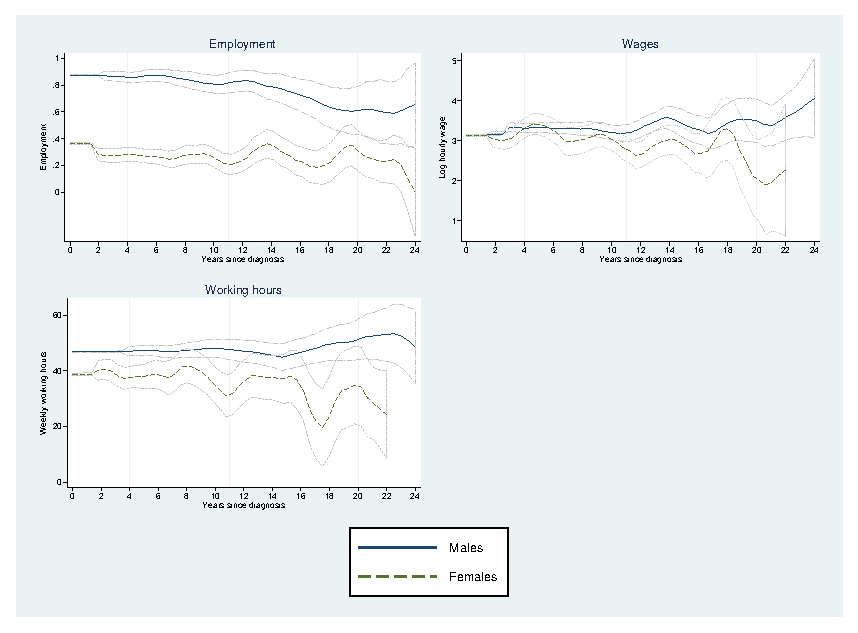
\includegraphics[width=\linewidth]{figures/lpoly_combined.eps}\\
		\footnotesize{\textit{Notes} The dashed lines show 95\% confidence intervals.}
	\end{center}
\end{figure}


\begin{figure}[h!]
	\caption{\label{fig:kdens_inconsistency_hba1c}Kernel density of HbA1c values for those with one inconsistent and two inconsistent reports.}%
	\begin{center}
		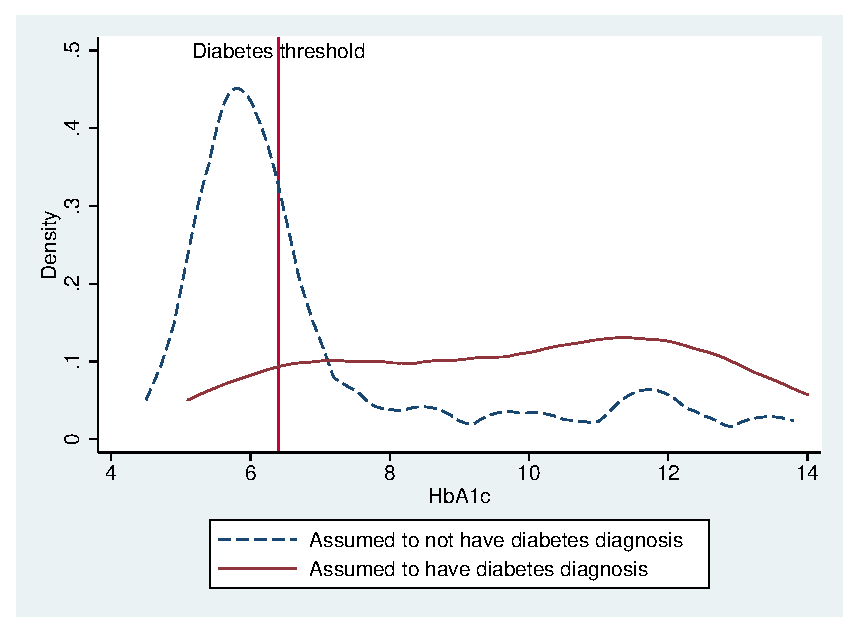
\includegraphics[width=.5\linewidth]{figures/kdensity_hba1c_inconsist.eps}\\
	\end{center}
\end{figure}

\end{document}

